\documentclass[multi,tikz,crop=false,class=article]{standalone}

\onlyifstandalone{\usepackage{hyperref}
\usepackage{cleveref}
\usepackage[disable]{todonotes}
\presetkeys{todonotes}{inline, noline}{}
\usepackage{caption}
\usepackage{subcaption}
\usepackage{amsfonts}
\usepackage{theorem}
\usepackage{algorithm}
\usepackage{algpseudocode}
\theoremstyle{plain}
\theorembodyfont{\slshape}
\newtheorem{definition}{Definition}[section]
\usepackage{algorithm}
\usepackage{algpseudocode}
\usepackage{amsmath}
\usepackage{mathtools}
\usepackage{tikz}

\usetikzlibrary{automata,arrows}

%\DeclareCaptionType{algorithm}
\algdef{SE}[DOWHILE]{Do}{doWhile}{\algorithmicdo}[1]{\algorithmicwhile\ #1}%

% Math macros
\newcommand{\concat}{\cdot}
\newcommand{\bool}{\ensuremath{\mathbb{B}}}
\newcommand{\lang}{\ensuremath{\mathcal{L}}}
\newcommand{\dstar}[2]{\ensuremath{\delta^*(#1,#2)}}
\newcommand{\exec}[2]{\ensuremath{#1[#2]}}
\newcommand{\access}[2]{\ensuremath{#1^{-1}[#2]}}
\newcommand{\nero}{\ensuremath{\equiv}}
\newcommand{\eqclass}[2]{\ensuremath{[#1]_{#2}}}
\newcommand{\mq}{\ensuremath{\mathsf{member}}}
\newcommand{\eq}{\ensuremath{\mathsf{equiv}}}
\newcommand{\row}{\ensuremath{\mathsf{row}}}
\newcommand{\sift}{\ensuremath{\mathsf{sift}}}
%%% Local Variables:
%%% mode: latex
%%% TeX-master: t
%%% End:
}
\onlyifstandalone{\usepackage{mathtools}}
\onlyifstandalone{\usepackage{algpseudocode}}
\onlyifstandalone{\DeclareCaptionType{algorithm}}

\usetikzlibrary{automata,arrows}
\algdef{SE}[DOWHILE]{Do}{doWhile}{\algorithmicdo}[1]{\algorithmicwhile\ #1}%

\begin{document}
\section{Variants}
\label{sec:variants}
In the first few years following the introduction of the $L^*$ algorithm by
Angluin~\cite{Angluin1987}, $L^*$ learning was only a theoretical exploration.
The various improvements described in the previous chapter,
such as \textit{Classification Trees} \cref{sec:classification-trees} and
the \textit{TTT} algorithm \cref{sec:ttt} made practical applications more feasible.

The learning algorithms discussed in the previous chapters all required an
(abstract, formal) input alphabet, an (abstract, formal) output alphabet,
membership queries and equivalence queries.
In practice, it is in many cases quite difficult to realize these requirements
for a specific system under learning (SUL)~\cite{Steffen2011a}.
This section discusses some of these challenges faced when
applying active state machine learning to real world scenarios, such as:
\begin{itemize}
  \item Equivalence queries are generally undecidable for black box systems.
  \item The amount of required membership queries can grow very fast,
        possibly making applications of $L^*$ learning very time consuming.
  \item $L^*$ can only interact with regular languages, not with real systems.
  \item $L^*$ assumes that the SUL can always return to its initial state,
        imposing the requirement that membership queries are independent.
        In practice the SUL might not be able to do so,
        which results in the requirement of a \textit{reset} function.
        However, not all systems support a \textit{reset} function.
\end{itemize}
For each of these challenges a variant of the $L^*$ algorithm will be discussed
that addresses the specific issues encountered.

\subsection{Approximating $\eq(M)$ queries with $\mq(w)$ queries}
In theoretical simulations, equivalence testing is often easy because
the target system (in some cases even the model!) is known.
In practice, however, the system under learning is generally
a black box, since the main motive for using a learning algorithm is to
infer knowledge about some unknown system.
Therefore equivalence queries can generally only be answered by exhaustively
testing the inputs and outputs of a system.
However, exhaustively testing a black box is undecidably hard.

This means that equivalence queries will have to be approximated,
typically using membership queries. These approximated equivalence queries are in
general also not decidable without assuming any extra knowledge~\cite{Steffen2011a},
such as the number of states of the system under learning: it is impossible to
be certain that the system has been tested extensively enough.

An alternative to using equivalence queries, is to use model-based testing
methods~\cite{Broy2005, Tretmans2011}. An example of
model-based testing is Chow's W-method~\cite{deRuiter2015, Chow1978},
which relies on approximating $\eq(M)$ queries by using $\mq(w)$ queries.

%To further research in this area,
%the \textit{ZULU} challenge~\cite{Combe2010} was introduced.
%The \textit{ZULU} challenge asked participants to find a DFA corresponding
%to a certain system as accurately as possible, while imposing a restriction
%on the number of \textit{MEMBER (w)} queries and disallowing \textit{EQUIV (M)}
%queries completely.
%\todo{add some more text and a fluid intro to Chow's method}

\subsubsection{Chow's W-method}
\label{sec:chow}
According to~\cite{Vasilevskii1973}, the maximum number of test sequences needed
to converge to a correct approximation of the system under learning
is bounded by $n^{2} \times k^{m-n+1}$ when using Chow's W-method.
The maximum length of these sequences is $n^{2} \times m \times k^{m-n+1}$,
where $n$ is the number of states in the provided automaton, $m$ is the number
of states in the correct automaton and $k$ is the size of the input alphabet.

By refining the test suites and the specification at the same time
and by using a divide and conquer approach, the size of the test is
considerably reduced in comparison to defining the tests from
the final specification~\cite{Ipate2007, Chow1978}.
This is especially beneficial because complex systems are usually
created in multiple iterations.
Unlike some other test selection methods the W-method does not require
that the number of states is exactly the same between
the implementation and protocol.
The W-method generates tests that guarantee correctness of an
implementation with a number of states below a certain upper bound.

The W-method generates input sequences that reach every state in the
diagram, checks all the transitions in the diagram and identifies all the
destination states and verifies them against their counterparts in
the implementation~\cite{Ipate2007}.
To achieve this, the W-method constructs two sets of input sequences:
\begin{itemize}
  \item A state cover $S \subseteq \Sigma^{*}$ that reaches every state in the
    final state machine, including the empty sequence to reach the initial state.
  \item A characterization set $W \subseteq \Sigma^{*}$ that has different
    outputs for at least one sequence in $W$ for every pair of different states.
\end{itemize}

Given a specification $P$ that can be modeled by an unknown finite state machine $M$,
the only information the algorithm needs is an estimate of the maximum number of
states of an unknown model for the specification.
Suppose $d$ is the difference between the estimated maximum number of states in $P$
and the number of states in the machine $M$.
We also take $\Sigma \left[ n \right] = \Sigma^{n} \cup \dots \cup \lbrace \epsilon \rbrace$,
making $\Sigma\left[ n \right]$ a random string with a maximal length of $n$.
For the W-method the testing suite $T = S \concat \Sigma\left[ d + 1 \right]  \concat W$.
The idea behind the W-method is that $S \concat \Sigma\left[ 1 \right]  = S \cup (S
\concat \Sigma)$, which is also called the transition cover of $M$, ensures that all the
states and transition in $P$ are also present in $M$, while
$\Sigma\left[ n \right] \concat W$ ensures that $M$ and $P$ are in the same state after
performing all the transitions.

\subsection{Limiting the amount of membership queries}
Membership queries are the most straightforward
to translate to real world applications: they can be realized via testing.
An important thing to note, however, is the amount of membership queries required.
In a theoretical framework the learning algorithm does not have to account
for execution times of individual $\mq(w)$ queries.
In practice, such queries might take considerable time or be expensive to execute.

Learning a real world application can easily require several thousand membership
queries~\cite[p. 100]{Tomte2014}. Furthermore, when using for example
\textit{Chow's method} for $\eq(M)$ queries, the amount of membership
queries needed grows exponentially in the number of states~\cite{Chow1978}.
This means that the time required to learn a model can be greatly reduced
either by speeding up membership queries
(executing them in parallel~\cite{Howar2012}),
or simply by reducing the number of membership queries required~\cref{sec:tools}.

\todo{Needs expansion, see todo list in issues}
Chapter \ref{sec:improvements} has discussed several improvements to achieve
exactly that. Additionally, application-specific optimizations can be used to
further reduce the number of membership queries required.
When dealing with a networked application for example, there are usually no
further possible transitions when a connection is closed by a remote machine.
Exploiting such knowledge can greatly reduce the number of tests necessary~\cite{deRuiter2015}.

%\todo{Cite ZULU participant here, since the challenge also imposed
%      a maximum on \textit{MEMBER (w)} queries}

\subsection{Learning Mealy machines}
\label{sec:learn-mealy-mach}

The $L^*$ algorithm of Angluin is only able to learn DFAs (and equivalent
models). However, some applications are characterized by their I/O behavior.
Such behavior is not easily modeled by a DFA. Instead, they are more naturally
modeled by Mealy machines\cite{Shahbaz2009} (see definition
\ref{def:mealy_machine}).

\begin{definition}[Mealy machine]\label{def:mealy_machine}
  A Mealy machine $M$ is a 6-tuple $(Q, q_0, \Sigma, \Lambda, \delta, \lambda)$
  where $Q$ is the set of states, $q_0$ is the initial state, $\Sigma$ is the
  input alphabet, $\Lambda$ is the output alphabet, $\delta$ is the transition
  function and $\lambda$ is the output function.
\end{definition}

A Mealy machine is similar to a DFA, but instead of defining accepting states,
it defines a function $\lambda: Q \times \Sigma \to \Lambda$ that defines
the output symbol returned on each state transition. To learn a Mealy machine
with $L^*$, some adaptions are required: either the Mealy machine can be
transformed into a DFA, or an adaptation of $L^*$ called $L^*_{M}$ can be used
to learn the Mealy machine directly.

\subsubsection {Transforming a Mealy machine into a DFA}

A Mealy machine $\mathcal{M}$ can be transformed into a DFA $D$. By using the
alphabet of the transformed model, $D$ can be learned by the $L^*$ algorithm.
The only required change to the algorithm is the implementation of the
membership query, as will be explained below. There are two ways to transform
$\mathcal{M}$ into $D$. Both transformations have in common that they introduce
a single error state $q_{err}$, which is the only non-accepting state in $D$.
The main difference between the transformations is in the input alphabet they
define. One uses $\Sigma = \Sigma_\mathcal{M} \cup \Lambda$\cite{Hungar2003},
while the other uses $\Sigma = \Sigma_\mathcal{M} \times O$ \cite{Makinen2001}.
Note that in this section the $_{\mathcal{M}}$ subscript is used to disambiguate
between items from the DFA and Mealy tuples.


When using $\Sigma = \Sigma_\mathcal{M} \cup \Lambda$, each transition in
$\mathcal{M}$ with input symbol $\sigma$ and output symbol $o$ is split into two
transitions. The first is constrained by $\sigma$ and transitions to a new
intermediate state $q_t$. The second transitions from $q_t$ and is constrained
by $o$. All inputs that are not defined after this step transition into
$q_{err}$. An example can be seen in figure \ref{fig:transformation_hungar} and
the pseudocode of this transformation is shown in algorithm
\ref{alg:transform_hungar}. The transformed model of $\mathcal{M}$ can be
learned by $L^*$ by defining $\Sigma = \Sigma_\mathcal{M} \cup \Lambda$
\cite{Shahbaz2009} and using the appropriate $\mq$ and $\eq$ implementations
\cite{Hungar2003,Niese2003}.

\begin{itemize}
  \item the first symbol is an input symbol;
  \item input and output symbols are alternating;
  \item for each successive pair of input symbol $\sigma$ and output symbol $o$
        in the access string, if $\sigma$ is applied, $o$ is returned;
\end{itemize}

\begin{algorithm}[h]
\caption{Transformation of a Mealy machine into a DFA}
\label{alg:transform_hungar}
\begin{algorithmic}[1]
\Function{Transform}{$Q_\mathcal{M}, q_{0_\mathcal{M}}, \Sigma_\mathcal{M},
                     \Lambda, \delta_\mathcal{M}, \lambda$}
  \State $Q \gets Q_\mathcal{M} \cup \{q_{err}\}$
  \State $q_0 \gets q_{0_\mathcal{M}}$
  \State $\Sigma \gets \Sigma_\mathcal{M} \cup \Lambda$
  \For{$(q,\sigma) \in Q_\mathcal{M} \times \Sigma_\mathcal{M}$}
  \Comment For each transition in $\mathcal{M}$
    \State add a new state $q_t$ to $Q$
    \State $\delta(q,\sigma) \gets q_t$
    \Comment Add a transition to $q_t$
    \State $\delta(q_t, \lambda(q,\sigma)) \gets \delta_\mathcal{M}(q, \sigma)$
    \Comment Add a transition from $q_t$
  \EndFor

  \For{$(q, \sigma) \in Q \times \Sigma$}
    \If{$\delta(q, \sigma)$ is not yet defined}
      \State $\delta(q, \sigma) \gets q_{err}$
    \EndIf
  \EndFor
  \State $F \gets Q - \{q_{err}\}$
  \State \Return $(Q, q_0, \Sigma, \delta, F)$
\EndFunction{}
\end{algorithmic}
\end{algorithm}

\begin{figure}[t]
\centering
\begin{subfigure}[b]{.4\textwidth}
\centering
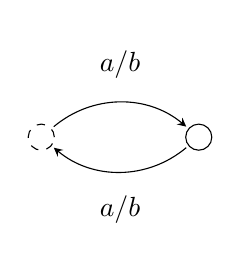
\begin{tikzpicture}
  [bend angle=40,every node/.style={draw,circle}]

  \tikzstyle{initial} = [dashed]

  \node[initial]   (1) at (1,0) {};
  \node        (2) at (3,0) {};

  \path[->, >=stealth, shorten > = 1pt, shorten < = 1pt]
        (1) edge [bend left] node[auto,draw=none] {$a/b$} (2)
        (2) edge [bend left] node[auto,draw=none] {$a/b$} (1);
\end{tikzpicture}
\caption{Mealy representation} \label{fig:transformation_mealy}
\end{subfigure}
\hfill
\begin{subfigure}[b]{0.4\textwidth}
\centering
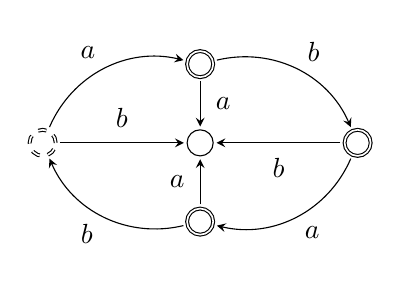
\begin{tikzpicture}
  [bend angle=40,every node/.style={draw,circle}]

  \tikzstyle{initial} = [dashed]

  \node[initial, accepting] (1) at (1,0)  {};
  \node                     (2) at (3,0)  {};
  \node [accepting]         (3) at (5,0)  {};
  \node [accepting]         (4) at (3,-1) {};
  \node [accepting]         (5) at (3,1)  {};

  \path[->, >=stealth, shorten > = 1pt, shorten < = 1pt]
        (1) edge [bend left] node[auto,draw=none] {$a$} (5)
        (4) edge [bend left] node[auto,draw=none] {$b$} (1)
        (5) edge [bend left] node[auto,draw=none] {$b$} (3)
        (3) edge [bend left] node[auto,draw=none] {$a$} (4)
        (1) edge 			 node[auto,draw=none] {$b$} (2)
        (3) edge 			 node[auto,draw=none] {$b$} (2)
        (4) edge 			 node[auto,draw=none] {$a$} (2)
        (5) edge 			 node[auto,draw=none] {$a$} (2);
\end{tikzpicture}
\caption{Hungar's transformation} \label{fig:transformation_hungar}
\end{subfigure}

\caption{Mealy to DFA transformation} \label{fig:transformation}
\end{figure}

The second transformation uses $\Sigma = \Sigma_\mathcal{M} \times \Lambda$.
M\"{a}kinen~et~al were the first to use (a slightly modified version of) $L^*$
to learn a DFA with input/output pairs as input symbols. Several other papers
mention that a DFA with such inputs can be created from a Mealy machine by
taking $\Sigma = \Sigma_\mathcal{M} \times \Lambda$, and that therefore Mealy
machines can be learned by $L^*$ \cite{Shahbaz2009,Irfan2010,Groz2012}. This
transformation removes the need for intermediate states, but it has significant
impact on the size of the input alphabet \cite{Hungar2003}. Since none of the
mentioned papers explicitly define the transformation in detail, no pseudocode
is given here.

\subsubsection {Adapting $L^*$ into $L^*_{M}$}
Angluin's $L^*$ algorithm has been adjusted for use with Mealy machines. The new
procedure was first informally described in \cite{Margaria2004}, and later more
rigorously in \cite{Shahbaz2009}. In $L^*$ the membership queries return a
boolean value; either it's a member, or it's not. For $L^*_{M}$, the membership
query is replaced by an output query, which returns an output string. The
observation table is modified to store these output strings instead of boolean
values. As in $L^*$, output queries are used in order to fill in the observation
table. Suppose the algorithm performs an output query for $s \concat e$, where
$s \in S \cup (S \concat \Sigma)$ and $e \in E$. The query will produce a string
$r$ with $|r| = |s| + |e|$, where $|x|$ denotes the length of the string $x$.
Instead of storing $r$ directly in the observation table, only the last $|e|$
symbols of $r$ are stored (since the observation is prefix closed, the output
corresponding to $s$ is already stored in the table). The intuitive meaning of
this value in the observation table is that it correspond to the sequence of
output symbols that is produced when the input $e$ is applied from the state
corresponding to $s$.

An example Mealy machine $\mathcal{M}$ is shown in figure
\ref{fig:mealy_example}. A possible observation table built by $L^*_M$ when it
learns $\mathcal{M}$ is shown in table \ref{tbl:mealy_observation_table} (source
of the example: Shahbaz~et~al \cite{Shahbaz2009}). In this table it can be seen
that the value in $\row(aa)$ under the column labeled by $a$ is $y$, even though
the output query would have returned the string $xyy$ for the input string
$aaa$.

With the new meaning of the values in the table, a value of $\epsilon$ in $E$
becomes nonsensical. This is because $\epsilon$ would denote no change in
state, so there would be no output symbol. Therefore, at the start of the
algorithm, $E$ is not intialized to $\{\epsilon\}$ but to $\Sigma$.

The concepts of closedness and consistency remain identical. The procedure to
build the hypothesis remains largely the same, but now the generated hypothesis
no longer defines accepting states, but instead defines output strings on the
transitions. Following similar reasoning as in Angluin's paper
\cite{Angluin1987}, it can be concluded that $L^*_M$ is guaranteed to find a
model describing the target using at most $\mathcal{O}(k^2nm + kmn^2)$ output
queries \cite{Shahbaz2009}.

\begin{figure}[h]
  \begin{minipage}{.45\textwidth}
    \centering
    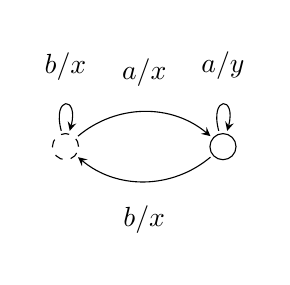
\begin{tikzpicture}
      [bend angle=40,every node/.style={draw,circle}]

      \tikzstyle{initial} = [dashed]

      \node[initial]   (1) at (1,0) {};
      \node        (2) at (3,0) {};

      \path[->, >=stealth, shorten > = 1pt, shorten < = 1pt]
            (1) edge [bend left] node[auto,draw=none] {$a/x$} (2) 
            (2) edge [bend left] node[auto,draw=none] {$b/x$} (1)
            (1) edge [loop above] node[auto,draw=none] {$b/x$} (1)
            (2) edge [loop above] node[auto,draw=none] {$a/y$} (2);
    \end{tikzpicture}
    \captionof{figure}[t]{Example Mealy machine}
    \label{fig:mealy_example}
  \end{minipage}
%
  \begin{minipage}{.45\textwidth}
    \centering
    \begin{tabular}{ | l || c | c | }
      \hline
                  & $a$   & $b$ \\ \hline \hline
      $\epsilon$  & $x$   & $x$ \\ 
      $a$         & $y$   & $x$ \\ \hline \hline
      $b$         & $x$   & $x$ \\
      $aa$        & $y$   & $x$ \\
      $ab$        & $x$   & $x$ \\
      \hline
    \end{tabular}
    \captionof{table}[t]{Example observation table}
    \label{tbl:mealy_observation_table}
  \end{minipage}
\end{figure}


\subsection{Systems without a \textit{reset} function}
\label{sec:noreset}
In the $L^*$ learning algorithm, every $\mq(w)$ query is implicitly
independent of other queries.
However, when learning a system in practice, it might happen that
$\mq(w)$ queries are not independent at all.
Suppose for example that the system under learning requires authentication
while also imposing a restriction on the maximum amount of failed requests.
In such a system queries are no longer independent of each other,
since after a certain amount of authentication requests
the systems behavior suddenly changes for the same membership queries.
In order to solve this issue, the $L^*$ algorithm implicitly requires a means
of resetting the system under learning~\cite[p. 301]{Rivest1993}
in between successive membership queries.

However, not in all situations a reset function is desirable. An example is a
system where the reset takes a lot of time compared to the learning process.
For such systems a reduction in the amount of resets is helpful. The method
proposed by Bauer~et~al.~\cite{Bauer2012} can be used for this situation. This
method reuses already (or partially) asked membership queries by only sending
the remaining part of the query to the teacher. It then combines the answer of
the teacher (if needed) with the answer of previously asked queries, which is
sent back to the learning algorithm. The system then only needs to reset if the
complete membership query has not already been asked before.
Other systems lack any support for a reset function.
As we'll see in \cref{sec:applications}, the system under learning
could well be a system over which the algorithm has no control.

%Section 3.5?
%Another obstacle to overcome is that of parameters used in real world
%applications. Think, for example, about increasing sequence numbers in
%communication protocols. This is still a huge challenge to
%resolve~\cite{Steffen2011a} and for now, besides the creation of prototypical
%solutions~\cite{Aarts2010,Shahbaz2007,Howar2010},
%application-specific solutions have to be applied~\cite{Steffen2011a}.

\subsubsection{Homing sequences}
In 1993 Rivest \& Schapire proposed an extension to $L^*$~\cite[p. 312]{Rivest1993}
that replaces the implicitly required reset by homing sequences.
A homing sequence is an input string for which the automaton is guaranteed to
produce a sequence of outputs that completely determines the final reached state.
The sequence of outputs on input $w$ starting from a state $q$ is denoted as
$q \langle w \rangle$.
Now suppose $M$ is a DFA. A homing sequence $h$ for $M$ with outputs $s$ is then
a sequence of strings, such that $(\forall{q_1 \in Q})(\forall{q_2 \in Q})
(q_1 \langle h \rangle = q_2 \langle h \rangle = s)$.

This also implies that every distinguisting sequence is a homing sequence,
since for all states $q_1$ and $q_2$ and a distinguishing extension $a$,
it can be deduced that $\delta(q_1, a) = \delta(q_2, a) \Rightarrow q_1 = q_2$
and therefore $q_1 \langle a \rangle = q_2 \langle a \rangle$.

Given this definition of a homing sequence, together with the prerequisite
that some state with outputs $s$ can be reached regularly by executing $h$,
it can immediately be seen how a homing sequence can be used to simulate a reset:
\begin{algorithm}[hb]
  \caption{Simulate a reset of the system with a homing sequence.}
  \label{alg:reset-homing}
  \begin{algorithmic}[1]
    \Function{Reset}{$M,h,s$} \Comment{With $M$ a DFA, $h$ a homing sequence and $s$ a sequence of outputs}
      \Do
        \State $o \gets $ result of executing $h$ on $M$
      \doWhile{$o \neq s$}
    \EndFunction{}
  \end{algorithmic}
\end{algorithm}

From the definition, given a homing sequence $h$, the state that is reached
by executing $h$ can be identified by a sequence of outputs $s$.
Therefore the algorithm can just execute $h$ for as long as its sequence of
outputs differs $o$ from $s$ and eventually the state identified by $s$ will be reached.
The $L^*$ algorithm can now just substitute its initial state with the state
reached eventually by executing $h$, giving it the ability to simulate a reset.

With every string there is the possibility that $M$ gets trapped in a loop.
Therefore it is generally quite hard if not impossible to find such a state.
Rivest \& Schapire solve this by simulating independent copies of $M$
for each possible output $s$ on executing $h$~\cite[p. 313]{Rivest1993}.
Since the set of possible outputs on $h$ is limited by the number of states $n$,
the amount of independent copies is bounded by $\mathcal{O}(n)$.
Therefore this algorithm is bounded by $\mathcal{O}(n \cdot (m + e))$,
with $m$ the amount of $\mq(w)$ queries and $e$ the amount of $\eq(M)$ queries.
\\
\\
All the above problems might give the impression that active state machine
learning is not yet applicable to real world applications. While it is true that
practical application is not yet complete, great progress has been made and
great things have already been achieved. The last chapter serves to highlight
some real world applications that illustrates these facts.

\end{document}

%%% Local Variables:
%%% mode: latex
%%% TeX-master: "main"
%%% End:
